\def\DoNotLoadEpstopdf{}
\documentclass[11pt]{article}
\usepackage{fontspec}
\setsansfont{texgyreheros-regular.otf}[BoldFont=texgyreheros-bold.otf]
\usepackage[paperwidth=21.85cm,paperheight=16.25cm,margin=0.55cm]{geometry}
\usepackage{tikz}
\usetikzlibrary{arrows.meta}
\pagestyle{empty}

\definecolor{ink}{HTML}{14263C}
\definecolor{muted}{HTML}{485C70}
\definecolor{blue}{HTML}{2D56A1}
\definecolor{teal}{HTML}{146B63}
\definecolor{amber}{HTML}{875017}

\begin{document}
\noindent
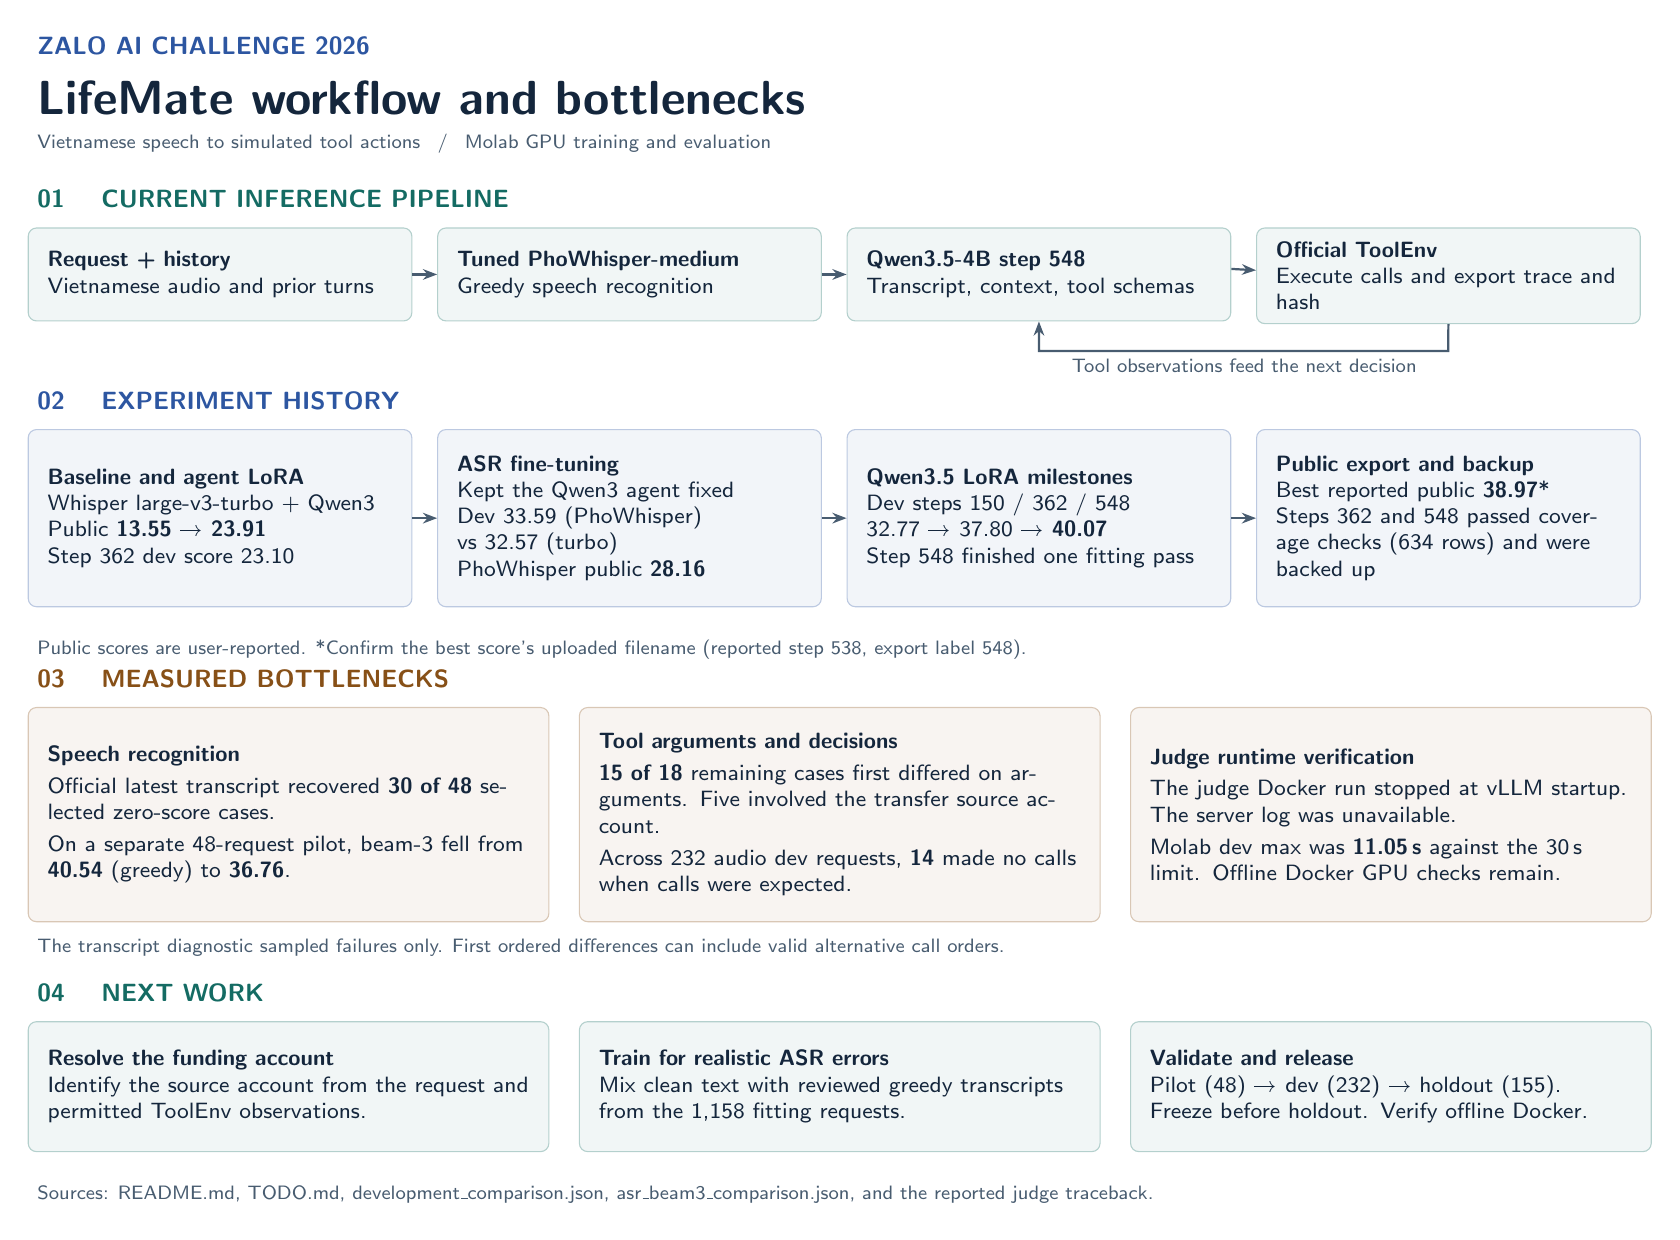
\begin{tikzpicture}[
  x=1cm,y=1cm,font=\sffamily,text=ink,
  section/.style={anchor=west,font=\sffamily\bfseries\small},
  note/.style={anchor=west,font=\sffamily\scriptsize,align=left,text=muted},
  card/.style={draw=#1!32,fill=#1!6,rounded corners=3pt,
    align=left,anchor=north west,inner xsep=7pt,inner ysep=5pt,font=\sffamily\footnotesize},
  stage/.style={card=teal,text width=4.38cm,minimum height=1.18cm},
  history/.style={card=blue,text width=4.38cm,minimum height=2.25cm},
  issue/.style={card=amber,text width=6.12cm,minimum height=2.72cm},
  next/.style={card=teal,text width=6.12cm,minimum height=1.65cm},
  flow/.style={-{Stealth[length=1.8mm]},draw=muted,thick},
]

\node[section,text=blue] at (0,0) {ZALO AI CHALLENGE 2026};
\node[anchor=west,font=\sffamily\bfseries\LARGE] at (0,-0.67)
  {LifeMate workflow and bottlenecks};
\node[note] at (0,-1.25)
  {Vietnamese speech to simulated tool actions \enspace / \enspace Molab GPU training and evaluation};

\node[section,text=teal] at (0,-1.95) {01 \quad CURRENT INFERENCE PIPELINE};
\node[stage] (audio) at (0,-2.31) {\textbf{Request + history}\\Vietnamese audio and prior turns};
\node[stage] (asr) at (5.2,-2.31) {\textbf{Tuned PhoWhisper-medium}\\Greedy speech recognition};
\node[stage] (agent) at (10.4,-2.31) {\textbf{Qwen3.5-4B step 548}\\Transcript, context, tool schemas};
\node[stage] (env) at (15.6,-2.31) {\textbf{Official ToolEnv}\\Execute calls and export trace and hash};
\draw[flow] (audio) -- (asr);
\draw[flow] (asr) -- (agent);
\draw[flow] ([yshift=2pt]agent.east) -- ([yshift=2pt]env.west);
\draw[flow] (env.south) -- (18.04,-3.88) -| (agent.south);
\node[note,anchor=north,inner sep=2pt] at (15.45,-3.9) {Tool observations feed the next decision};

\node[section,text=blue] at (0,-4.51) {02 \quad EXPERIMENT HISTORY};
\node[history] (base) at (0,-4.87)
  {\textbf{Baseline and agent LoRA}\\
   Whisper large-v3-turbo + Qwen3\\
   Public \textbf{13.55} → \textbf{23.91}\\
   Step 362 dev score 23.10};
\node[history] (tune) at (5.2,-4.87)
  {\textbf{ASR fine-tuning}\\
   Kept the Qwen3 agent fixed\\
   Dev 33.59 (PhoWhisper)\\
   vs 32.57 (turbo)\\
   PhoWhisper public \textbf{28.16}};
\node[history] (milestone) at (10.4,-4.87)
  {\textbf{Qwen3.5 LoRA milestones}\\
   Dev steps 150 / 362 / 548\\
   32.77 → 37.80 → \textbf{40.07}\\
   Step 548 finished one fitting pass};
\node[history] (release) at (15.6,-4.87)
  {\textbf{Public export and backup}\\
   Best reported public \textbf{38.97}*\\
   Steps 362 and 548 passed coverage checks (634 rows) and were backed up};
\draw[flow] (base) -- (tune);
\draw[flow] (tune) -- (milestone);
\draw[flow] (milestone) -- (release);
\node[note] at (0,-7.67)
  {Public scores are user-reported. *Confirm the best score's uploaded filename (reported step 538, export label 548).};

\node[section,text=amber] at (0,-8.04) {03 \quad MEASURED BOTTLENECKS};
\node[issue] at (0,-8.40)
  {\textbf{Speech recognition}\\[2pt]
   Official latest transcript recovered \textbf{30 of 48}
   selected zero-score cases.\\[2pt]
   On a separate 48-request pilot, beam-3 fell
   from \textbf{40.54} (greedy) to \textbf{36.76}.};
\node[issue] at (7.0,-8.40)
  {\textbf{Tool arguments and decisions}\\[2pt]
   \textbf{15 of 18} remaining cases first differed on arguments.
   Five involved the transfer source account.\\[2pt]
   Across 232 audio dev requests, \textbf{14} made no calls when calls were expected.};
\node[issue] at (14.0,-8.40)
  {\textbf{Judge runtime verification}\\[2pt]
   The judge Docker run stopped at vLLM startup.
   The server log was unavailable.\\[2pt]
   Molab dev max was \textbf{11.05\,s} against
   the 30\,s limit. Offline Docker GPU checks remain.};
\node[note] at (0,-11.46)
  {The transcript diagnostic sampled failures only. First ordered differences can include valid alternative call orders.};

\node[section,text=teal] at (0,-12.03) {04 \quad NEXT WORK};
\node[next] at (0,-12.39)
  {\textbf{Resolve the funding account}\\
   Identify the source account from the request and permitted ToolEnv observations.};
\node[next] at (7.0,-12.39)
  {\textbf{Train for realistic ASR errors}\\
   Mix clean text with reviewed greedy transcripts
   from the 1,158 fitting requests.};
\node[next] at (14.0,-12.39)
  {\textbf{Validate and release}\\
   Pilot (48) → dev (232) → holdout (155).\\
   Freeze before holdout. Verify offline Docker.};
\node[note] at (0,-14.59)
  {Sources: README.md, TODO.md, development\_comparison.json, asr\_beam3\_comparison.json, and the reported judge traceback.};
\end{tikzpicture}
\end{document}
